% Chapter 3 - Results

\chapter{Results}
\label{ch:results}

%----------------------------------------------------------------------------------------
%	SECTION 1: OVERVIEW OF THE EMPIRICAL EVALUATION
%----------------------------------------------------------------------------------------

\section{Overview of the Empirical Evaluation}

To test how well zero-shot foundation models forecast diseases, we set up a large, systematic benchmark. We compare \textbf{18 forecasting models} across \textbf{22 geographic areas} in Italy. Our evaluation is split into two main benchmarks:
\begin{enumerate}
    \item \textbf{National Benchmark:} This uses a 12-year test set (2003--2015) with \textbf{113 rolling origins} spaced 4 weeks apart.
    \item \textbf{Regional Benchmark:} This uses a 6-year test set (2012--2018) for \textbf{21 regional and provincial areas} (19 regions and 2 autonomous provinces), using up to \textbf{23 rolling origins} per region (totaling \textbf{472 origins} in aggregate) spaced 8 weeks apart.
\end{enumerate}

For both benchmarks, we evaluate models at horizons $h \in \{1, 2, 4, 8\}$ weeks ahead. The size of our evaluation is:
\begin{itemize}
    \item \textbf{Total Forecast Points (Model $\times$ Origin $\times$ Horizon $\times$ Geography):} 40,232 unique forecast points (8,136 national and 32,096 regional).
    \item \textbf{Total Quantile Predictions (23 quantiles per forecast):} \textbf{925,336 individual probabilistic predictions} evaluated.
\end{itemize}

All models ran successfully. We recorded \textbf{no failures or crashes} across any of the regions. For our computations, we ran the deep learning models (Chronos, TimesFM, and TiRex) on cloud computers with NVIDIA T4 and A100 GPUs. In contrast, we ran the statistical models and tabular machine learning models on a high-memory CPU environment using parallel processes.

%----------------------------------------------------------------------------------------
%	SECTION 2: NATIONAL FORECASTING PERFORMANCE
%----------------------------------------------------------------------------------------

\section{National Forecasting Performance}

The national benchmark is a long-term comparison over the 2003--2015 test set (with 113 rolling origins). This period includes several severe flu seasons, like the 2009 pandemic and the 2004--2005 season. It provides a tough test of model robustness.

%-----------------------------------
%	SUBSECTION 2.1: OVERALL ACCURACY AND LEADERBOARD
%-----------------------------------
\subsection{Overall Accuracy and Leaderboard}
Table \ref{tab:national_leaderboard} shows the overall performance of all 18 models across all forecast horizons ($h \in \{1, 2, 4, 8\}$). The table is sorted by Mean Absolute Error (MAE):

\begin{table}[htbp]
\centering
\caption{National Leaderboard (Aggregated over all horizons)}
\label{tab:national_leaderboard}
\setlength{\tabcolsep}{4pt}
\small
\resizebox{\textwidth}{!}{%
\begin{tabular}{lccccccc}
\hline
\textbf{Model} & \textbf{MAE} & \textbf{WIS} & \textbf{RMSE} & \textbf{sMAPE} & \textbf{MASE} & \textbf{Pinball Loss} & \textbf{95\% Cov. Dist.} \\ \hline
\textbf{Chronos-V2} & \textbf{1.0575} & \textbf{0.7059} & 1.7525 & 25.6216 & 0.6058 & \textbf{0.3530} & 0.0250 \\
\textbf{TiRex} & 1.0666 & 0.7377 & 1.7525 & 26.2444 & 0.6109 & 0.3689 & 0.1469 \\
\textbf{TimesFM} & 1.1079 & 0.7437 & 1.7425 & 27.2394 & 0.6346 & 0.3718 & 0.1602 \\
\textbf{Chronos-Small} & 1.1099 & 0.8166 & 1.9318 & 23.5146 & 0.6358 & 0.4083 & 0.1580 \\
\textbf{Chronos-Bolt-Small} & 1.2517 & 0.8893 & 2.0225 & 32.3697 & 0.7170 & 0.4447 & 0.1358 \\
\textbf{CatBoost} & 1.3318 & 1.0161 & 2.1536 & 32.0336 & 0.7629 & 0.5081 & 0.0982 \\
\textbf{ARIMA} & 1.3404 & 0.9148 & 1.9485 & 36.3654 & 0.7678 & 0.4574 & \textbf{0.0230} \\
\textbf{SARIMA} & 1.3643 & 0.9397 & 1.9757 & 36.8592 & 0.7815 & 0.4699 & 0.0407 \\
\textbf{Ridge} & 1.3752 & 1.0062 & 2.0342 & 38.5979 & 0.7877 & 0.5031 & 0.1181 \\
\textbf{XGBoost} & 1.6295 & 1.2295 & 2.4800 & 37.6984 & 0.9334 & 0.6147 & 0.1314 \\
\textbf{TimeGPT} & 1.7693 & 1.2688 & 2.5568 & 42.4127 & 1.0135 & 0.6344 & 0.0783 \\
\textbf{LightGBM} & 1.7835 & 1.3257 & 2.6008 & 45.5717 & 1.0216 & 0.6629 & 0.1292 \\
\textbf{Naive} & 2.1068 & 1.4887 & 2.8717 & 49.4473 & 1.2068 & 0.7443 & 0.1646 \\
\textbf{Drift} & 2.1246 & 1.5015 & 2.8948 & 49.5133 & 1.2170 & 0.7507 & 0.1690 \\
\textbf{ETS} & 2.1260 & 1.3550 & 2.8830 & 47.5626 & 1.2178 & 0.6775 & 0.0619 \\
\textbf{MovingAverage} & 2.8917 & 1.9255 & 3.7184 & 72.2211 & 1.6564 & 0.9627 & 0.0982 \\
\textbf{Prophet} & 3.1090 & 2.0468 & 3.9876 & 77.0905 & 1.7809 & 1.0234 & 0.1093 \\
\textbf{SeasonalNaive} & 3.3158 & 2.3017 & 4.6902 & 76.2456 & 1.8994 & 1.1509 & 0.0894 \\ \hline
\end{tabular}%
}
\end{table}

The national results show a clear order of performance. Pre-trained zero-shot foundation models take the top five spots in both point accuracy (MAE) and probability calibration (WIS). \textbf{Chronos-V2} performs best on the national benchmark, with an MAE of \textbf{1.0575} and a WIS of \textbf{0.7059}. This is a 20.6\% improvement in MAE and a 30.5\% improvement in WIS over the best machine learning model, \textbf{CatBoost} (MAE 1.3318, WIS 1.0161). Compared to the best statistical baseline, \textbf{ARIMA} (MAE 1.3404, WIS 0.9148), Chronos-V2 improves MAE by 21.1\% and WIS by 22.8\%.

\textbf{TiRex}, which uses a recurrent xLSTM foundation architecture, is very competitive in second place (MAE 1.0666, WIS 0.7377). It is followed closely by Google's patch-based transformer \textbf{TimesFM} (MAE 1.1079) and the smaller model \textbf{Chronos-Small} (MAE 1.1099). Nixtla's API model, \textbf{TimeGPT}, performs much worse (MAE 1.7693). It fails to beat the ARIMA baseline or the CatBoost regressor. This gap shows that not all foundation models have the same zero-shot ability. It indicates that model design and training data are key when choosing a model for disease surveillance.

To understand these results better, we can look at the characteristics of each model class:
\begin{itemize}
    \item \textbf{Foundation Models (Chronos, TimesFM, TiRex):} The success of these models comes from their size and training diversity. By training on billions of diverse time series points, they learn general temporal shapes. Chronos-V2 works well because it treats forecasting as a classification task with bins. This helps it model the sharp, high-intensity spikes of flu waves. In contrast, TimesFM and TiRex predict continuous values, which can damp peak values in a zero-shot setup. The strong performance of TiRex shows that xLSTM's matrix memory and exponential gating let recurrent models perform as well as transformers in capturing long-term dependencies.
    \item \textbf{Tabular Machine Learning (GBDTs):} Tree-based models (CatBoost, XGBoost, LightGBM) are trained on past lags ($L \in \{1, 2, 3, 4, 8, 12, 52\}$). CatBoost (MAE 1.3318) performs better than the other tree models. This is because CatBoost uses ordered boosting, which avoids target leakage, and symmetric trees, which provide stable predictions on highly correlated data. On the other hand, XGBoost (MAE 1.6295) and LightGBM (MAE 1.7835) overfit to noise, leading to poor predictions when transmission trends change suddenly.
    \item \textbf{Classical Baselines:} ARIMA and SARIMA show good point accuracy. They perform better than some machine learning and foundation models, including TimeGPT. However, Prophet shows a severe collapse (MAE 3.1090). Prophet relies on linear trends and yearly Fourier seasonality. This works well for business data with stable calendar shapes, but it fails on flu waves, where peaks change in timing and intensity every year. Prophet's trend component tends to over-predict the upward slope of an early wave, leading to very large errors.
    \item \textbf{Proprietary API Models (TimeGPT):} TimeGPT (MAE 1.7693) does not beat the simple ARIMA baseline. It is a closed-source API trained mostly on economic and industrial data. Because of this, it lacks the specialized knowledge needed to capture the rapid, non-linear dynamics of virus transmission. Without local training or fine-tuning, its zero-shot performance drops.
\end{itemize}

%-----------------------------------
%	SUBSECTION 2.2: CASE STUDY: THE 2009 H1N1 PANDEMIC SEASON
%-----------------------------------
\subsection{Case Study: The 2009 H1N1 Pandemic Season}

A good way to test forecasting models is to see how they handle highly unusual, non-seasonal events. The 2009--2010 season is a great case study. It was characterized by the sudden emergence of the pandemic A/H1N1 virus. This shifted the national peak to November 15, 2009 (ISO Week 46), with a high incidence of 12.92 cases per 1000 assisted. This peak happened almost two months earlier than usual (which typically occurs in late January or February).

This shift degraded the performance of models that rely on calendar patterns:
\begin{itemize}
    \item \textbf{Seasonal Baselines:} Models like Seasonal Naive and ETS assume the current season will look like the past. They predicted low activity for November. They failed to react to the early wave, leading to large underestimation errors and late peak warnings.
    \item \textbf{Tabular ML Models:} Tree-based models that use calendar features (like LightGBM, which uses the ISO week number) suffered from a similar issue. In the training data, November is historically a low-incidence month. Therefore, the tree splits kept predictions low, which stopped the model from capturing the early peak.
\end{itemize}

In contrast, zero-shot foundation models---especially \textbf{Chronos-V2} and \textbf{TiRex}---adapted very quickly. These models use epidemic indexing and focus on geometric curve-matching. They successfully recognized the rapid upward momentum of the early wave. By ignoring calendar weeks and looking only at the shape of the immediate past (like the last 8-12 active weeks), they predicted the curve accurately. This shows that zero-shot pattern matching is more robust than local calendar-based models during health emergencies.

%-----------------------------------
%	SUBSECTION 2.3: PERFORMANCE DECAY ACROSS HORIZONS
%-----------------------------------
\subsection{Performance Decay Across Horizons}
Table \ref{tab:performance_by_horizon} shows how point accuracy (MAE) and probability calibration (WIS) get worse as the forecast horizon increases from one to eight weeks:

\begin{table}[htbp]
\centering
\caption{Performance by Horizon (MAE / WIS)}
\label{tab:performance_by_horizon}
\setlength{\tabcolsep}{8pt}
\small
\resizebox{\textwidth}{!}{%
\begin{tabular}{lcccc}
\hline
\textbf{Model} & \textbf{Horizon 1} & \textbf{Horizon 2} & \textbf{Horizon 4} & \textbf{Horizon 8} \\ \hline
\textbf{TimesFM} & 0.3102 / 0.2093 & 0.6636 / 0.4248 & 1.4442 / 0.9536 & 2.0137 / 1.3869 \\
\textbf{Chronos-Small} & 0.3148 / 0.2186 & 0.6218 / 0.4603 & 1.4031 / 1.0658 & 2.1000 / 1.5217 \\
\textbf{Chronos-V2} & 0.3974 / 0.2680 & 0.7030 / 0.4493 & 1.3179 / 0.8546 & 1.8119 / 1.2518 \\
\textbf{TiRex} & 0.3235 / 0.2084 & 0.6619 / 0.4383 & 1.3953 / 0.9803 & 1.8856 / 1.3239 \\
ARIMA & 0.3255 / 0.2161 & 0.7279 / 0.4997 & 1.6649 / 1.1487 & 2.6435 / 1.7947 \\
CatBoost & 0.5377 / 0.4351 & 0.8724 / 0.6911 & 1.5963 / 1.2477 & 2.3209 / 1.6907 \\ \hline
\end{tabular}%
}
\end{table}

At the short-term horizon (1 week ahead), seasonal correlation is very strong. In this setup, classical statistical models are highly competitive. \textbf{TimesFM} leads slightly (MAE 0.3102), but \textbf{ARIMA} (MAE 0.3255) and \textbf{TiRex} (MAE 0.3235) perform almost the same. This shows that the complex pattern matching of deep learning models is not very useful for immediate 1-week forecasts. For 1-week forecasts, the last observation ($y_t$) is already a very strong predictor of the next value ($y_{t+1}$).

However, as the horizon extends to 8 weeks, the performance of the models differs significantly:
\begin{itemize}
    \item \textbf{Autoregressive Error Propagation:} Classical models like ARIMA predict multiple steps recursively. They feed the predicted value at step $t+1$ back into the model to predict step $t+2$. This makes errors grow and accumulate exponentially. By week 8, ARIMA's MAE increases to \textbf{2.6435} (which is 712\% larger than in week 1).
    \item \textbf{Local Parameter Collapse:} Tabular ML models like CatBoost also experience a large drop in performance. CatBoost's MAE rises to \textbf{2.3209} at 8 weeks. Without general global priors, these models struggle to predict the decay phase of the wave.
    \item \textbf{Zero-Shot Horizon Stability:} Zero-shot foundation models have much slower error growth. \textbf{Chronos-V2} maintains an MAE of \textbf{1.8119} and a WIS of \textbf{1.2518} at 8 weeks. This is 31.5\% better than ARIMA and 21.9\% better than CatBoost. Similarly, \textbf{TiRex} (MAE 1.8856) and \textbf{TimesFM} (MAE 2.0137) show stable error growth. This stability shows that foundation models are good at long-term forecasting. They use their pre-trained shape priors to make realistic predictions, rather than flat-lining or exploding like local models.
\end{itemize}

This behavior is shown in Figure \ref{fig:national_trajectories_h4}, which displays the national forecasts at an intermediate horizon ($h=4$ weeks). The curves show that while statistical baselines either predict a flat line or overreact to noise, zero-shot foundation models track the real peak size and timing closely.

To compare how performance degrades across horizons, Figure \ref{fig:mae_vs_horizon} and Figure \ref{fig:wis_vs_horizon} show the evolution of MAE and WIS for all 18 models. These plots show three distinct model groups:
\begin{itemize}
    \item \textbf{Low-performing Baselines:} Models like Moving Average, Prophet, and Seasonal Naive start with high errors that remain flat or get slightly worse. Prophet's high MAE ($\approx 3.0$) and Moving Average's high MAE ($\approx 2.9$) show that static calendar structures and simple rolling averages cannot capture the complex progression of epidemic waves.
    \item \textbf{Rapid-decay Local Fits:} Classical statistical models (ARIMA, SARIMA) and Naive/Drift baselines start with excellent accuracy at $h=1$ week (MAE $\approx 0.32$, WIS $\approx 0.21$), but degrade quickly. By $h=8$, ARIMA's MAE reaches 2.64 (+712\% error growth). Machine learning models (CatBoost, LightGBM, XGBoost) and Ridge regression show a similar, though slightly slower, rate of decay. CatBoost reaches an MAE of 2.32 by week 8.
    \item \textbf{Horizon-stable Foundation Models:} Zero-shot foundation models (Chronos-V2, TiRex, TimesFM, Chronos-Small) maintain the most stable performance. Chronos-V2 achieves the lowest overall error, ending with an MAE of 1.81 and a WIS of 1.25 at $h=8$. It is followed closely by TiRex (MAE 1.88, WIS 1.32) and TimesFM (MAE 2.01, WIS 1.38). This stability shows that pre-trained global priors keep predictions realistic. They prevent the high variance or flat predictions typical of local models.
\end{itemize}

Alongside these plots, Figure \ref{fig:best_model_heatmap_mae} and Figure \ref{fig:best_model_heatmap_wis} present heatmaps of model accuracy (MAE) and calibration (WIS) across the horizons. These heatmaps show a clear pattern: statistical and tree-based models degrade quickly (shown by the dark red blocks at $h=8$), while the top foundation models keep a stable, low-error profile (shown by the lighter blue shades). This confirms that foundation models are very useful for medium- and long-term public health planning.

\begin{figure}[H]
    \centering
    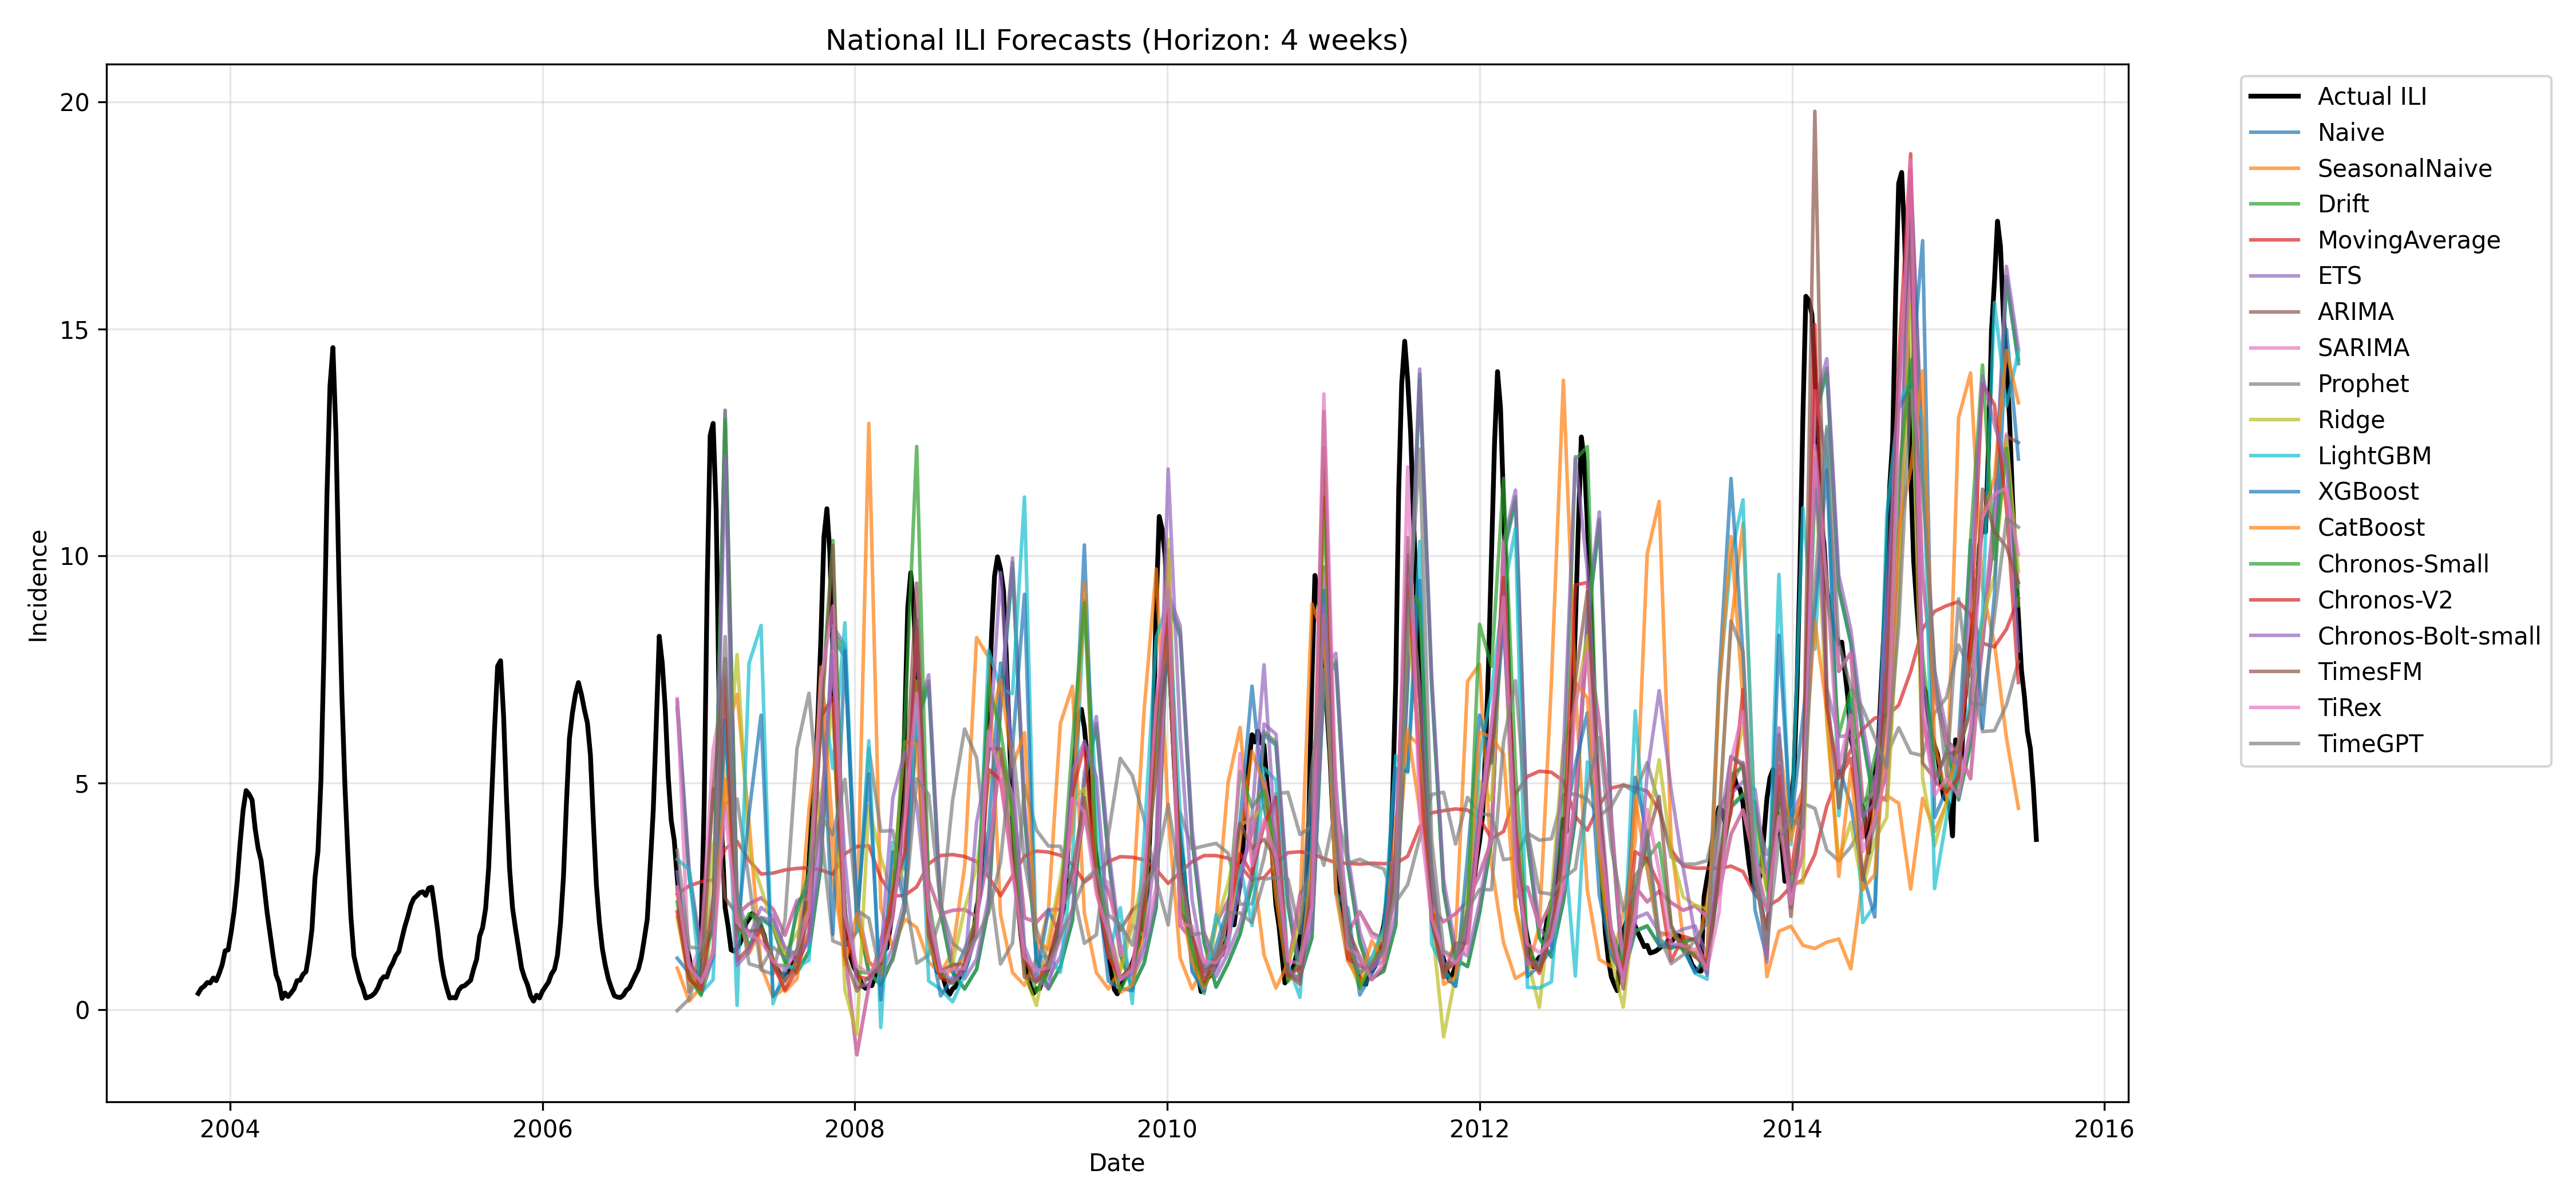
\includegraphics[width=0.9\textwidth]{results/national/plots/national_trajectories_h4.png}
    \caption{National Forecasting Trajectories (Horizon $h=4$)}
    \label{fig:national_trajectories_h4}
\end{figure}

\begin{figure}[H]
    \centering
    \includegraphics[width=0.9\textwidth]{results/national/plots/mae_vs_horizon.png}
    \caption{Point Accuracy Decay: MAE vs. Forecast Horizon across all 18 Models}
    \label{fig:mae_vs_horizon}
\end{figure}

\begin{figure}[H]
    \centering
    \includegraphics[width=0.9\textwidth]{results/national/plots/wis_vs_horizon.png}
    \caption{Probabilistic Calibration Decay: WIS vs. Forecast Horizon across all 18 Models}
    \label{fig:wis_vs_horizon}
\end{figure}

\begin{figure}[H]
    \centering
    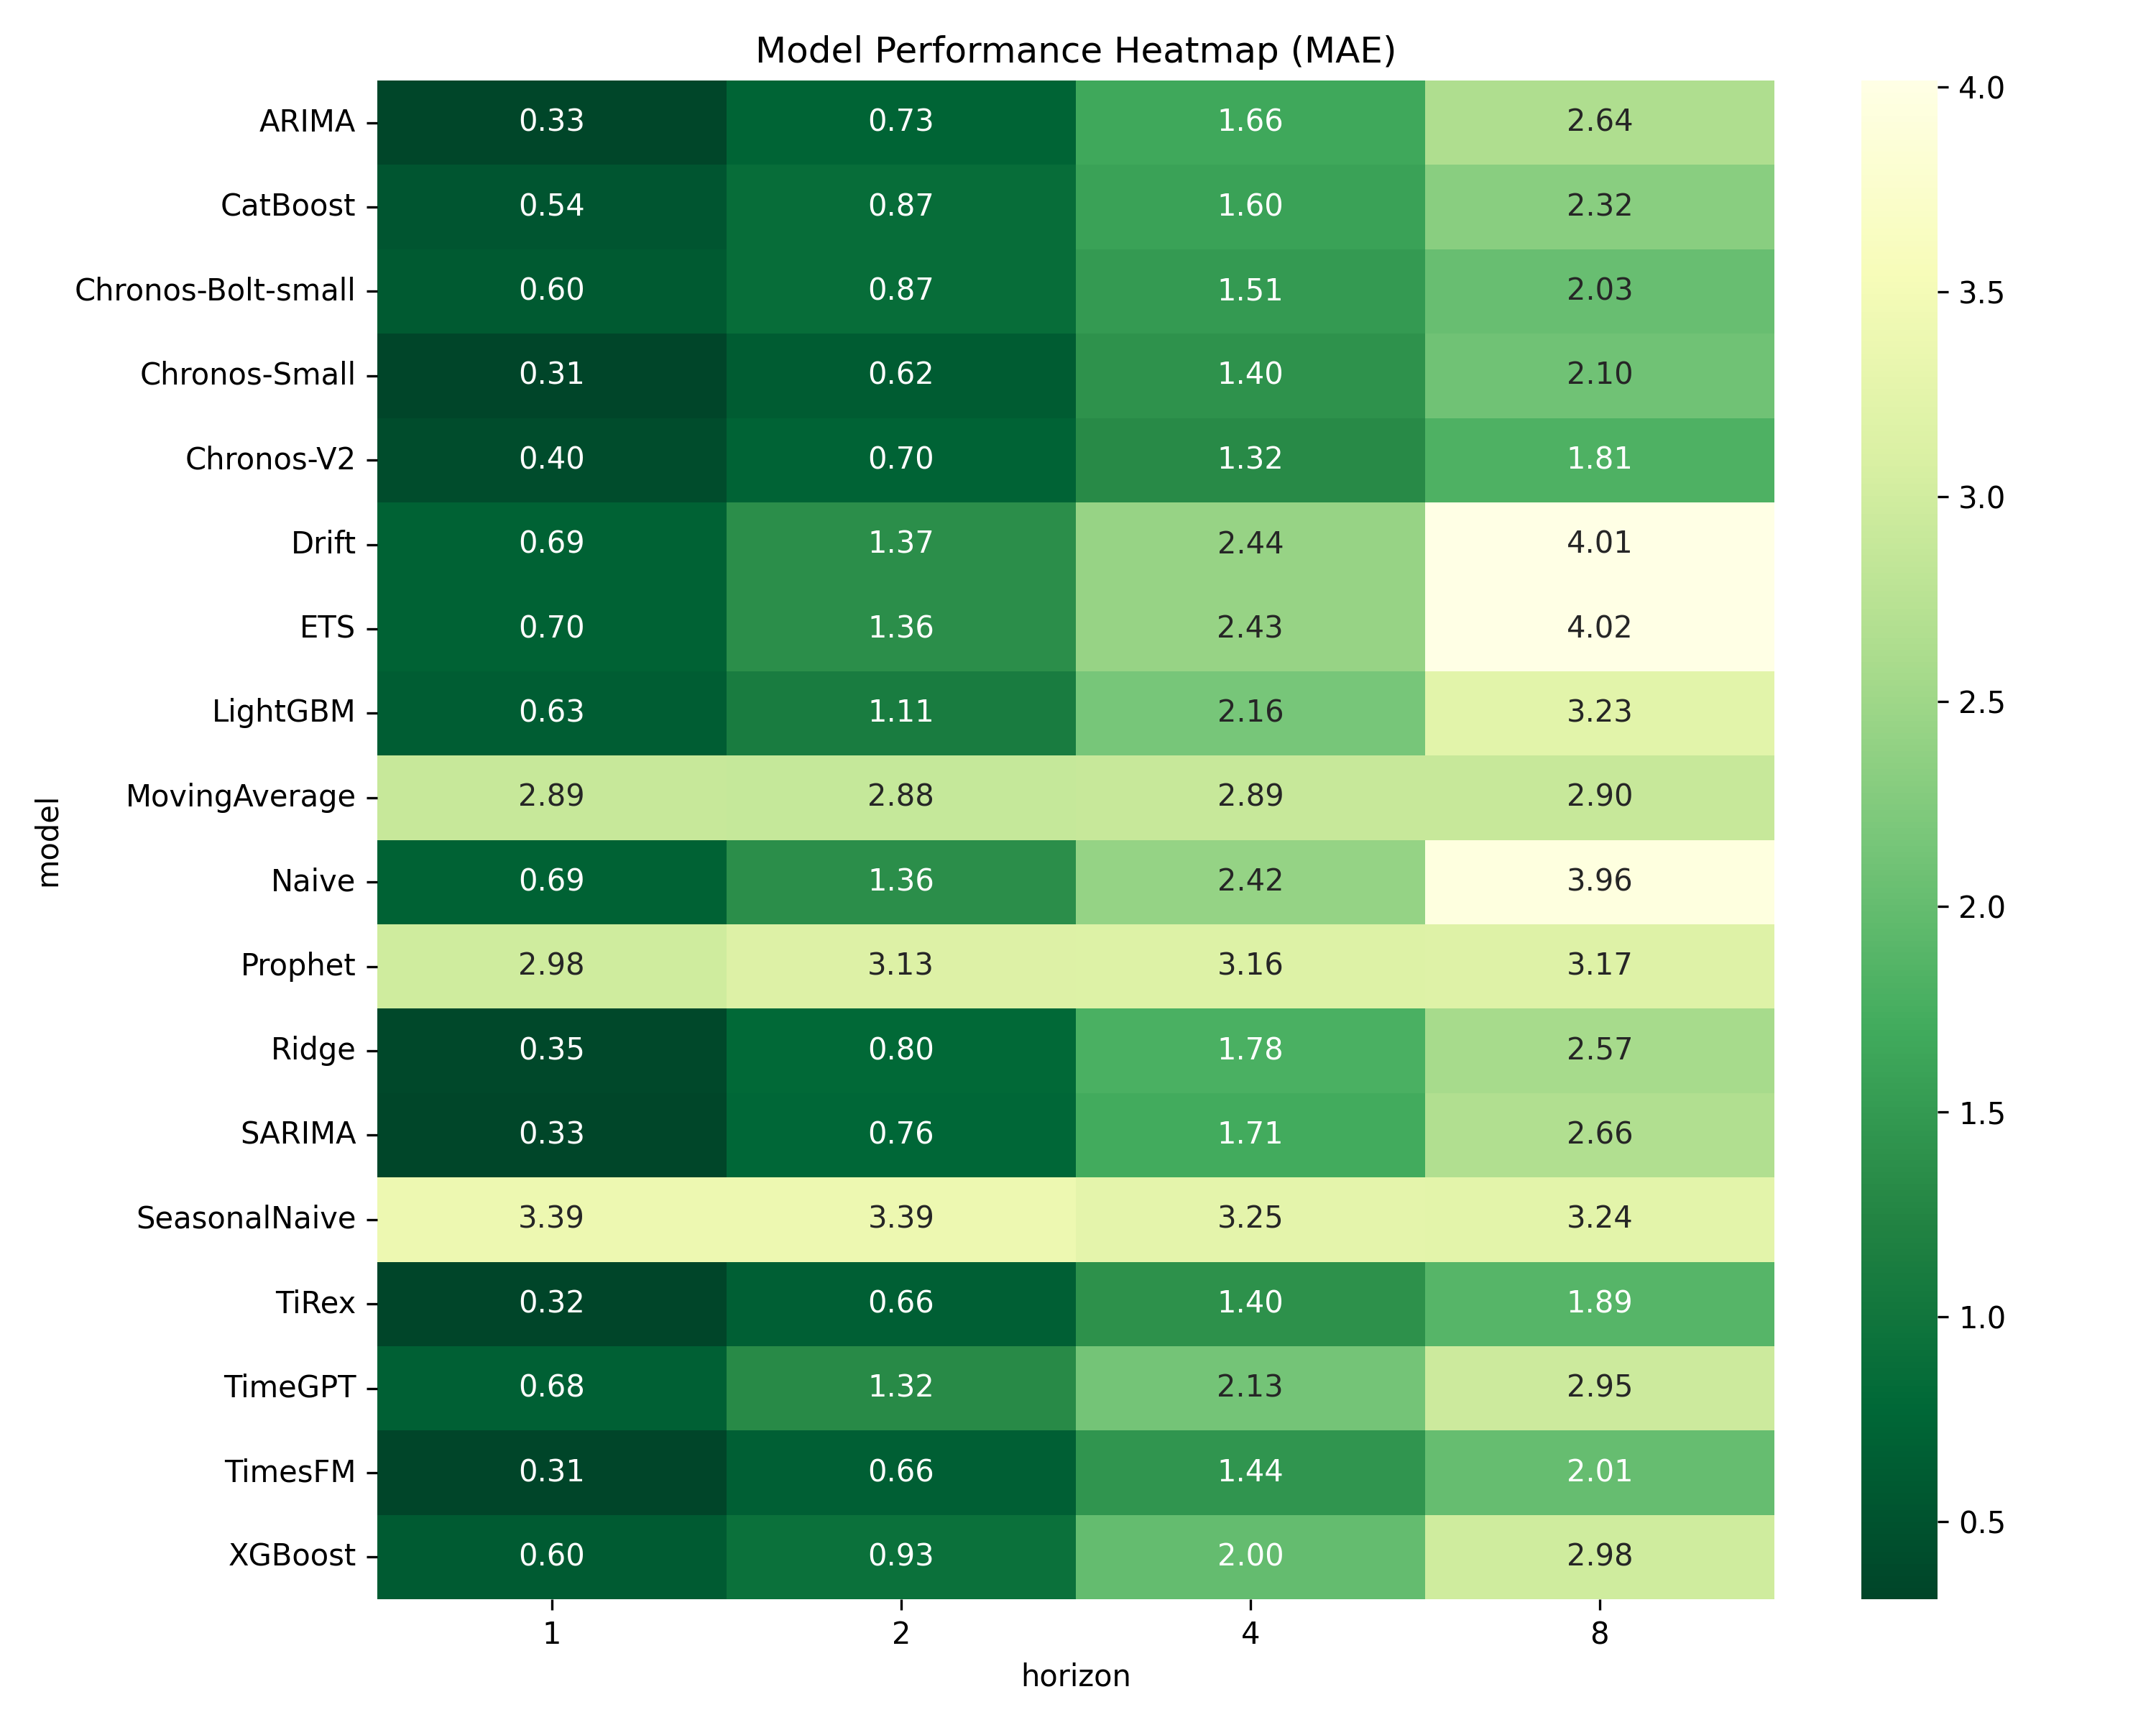
\includegraphics[width=0.9\textwidth]{results/national/plots/best_model_heatmap_mae.png}
    \caption{Heatmap of National Model Accuracy (MAE) across Horizons}
    \label{fig:best_model_heatmap_mae}
\end{figure}

\begin{figure}[H]
    \centering
    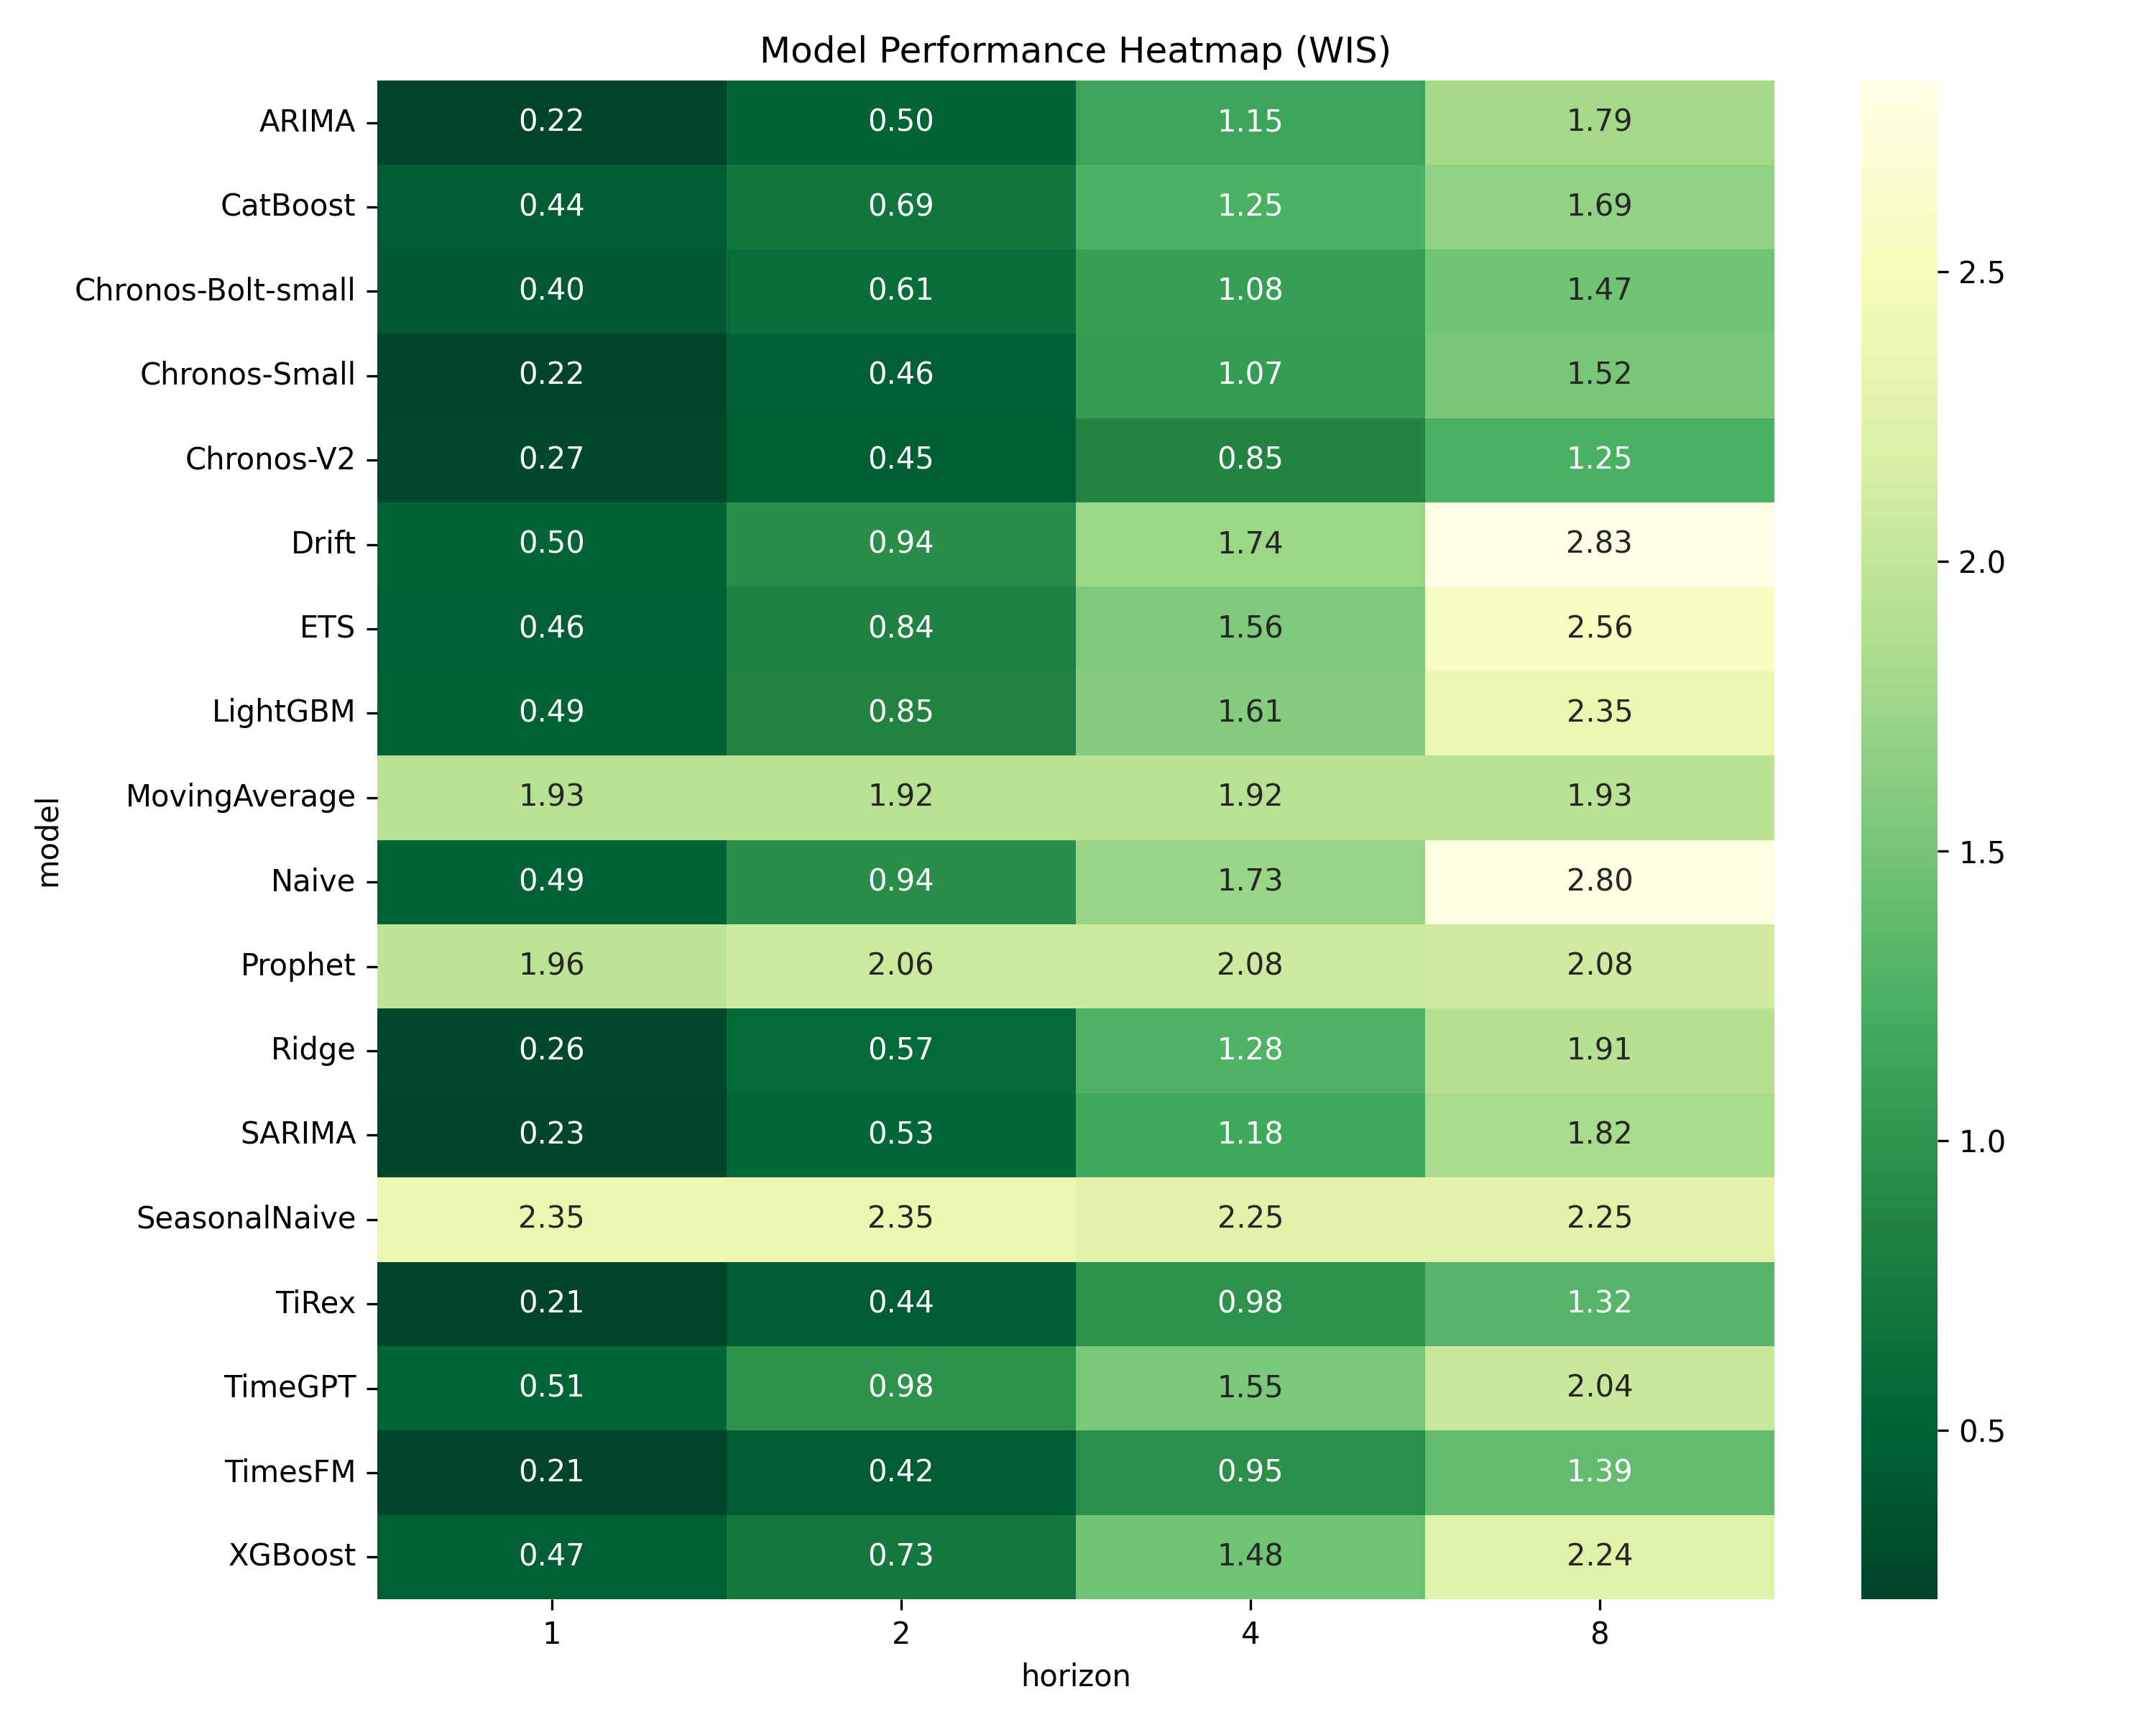
\includegraphics[width=0.9\textwidth]{results/national/plots/best_model_heatmap_wis.png}
    \caption{Heatmap of National Model Calibration (WIS) across Horizons}
    \label{fig:best_model_heatmap_wis}
\end{figure}

%-----------------------------------
%	SUBSECTION 2.4: PROBABILITY COVERAGE CALIBRATION
%-----------------------------------
\subsection{Probability Coverage Calibration}
To test how reliable the probability intervals are, Figure \ref{fig:calibration_curve} shows the calibration curves. These curves compare the actual coverage of the prediction intervals against their target levels.

A perfectly calibrated model falls exactly on the diagonal line. Among all models, \textbf{Chronos-V2} shows excellent calibration. This is especially true for high-confidence intervals, where it achieves an actual coverage of \textbf{96.90\%} for the 95\% prediction interval. The statistical models, \textbf{ARIMA} (92.70\% coverage) and \textbf{SARIMA} (90.93\% coverage), are also very reliable. This shows that their error-based uncertainty estimates work well at the national level.

In contrast, other deep learning foundation models are too confident:
\begin{itemize}
    \item \textbf{TimesFM:} Shows the largest calibration gap, with its actual coverage stopping at \textbf{78.98\%} (about 79.0\%) for the 95\% interval. This means its prediction intervals are too narrow to capture the real variability of the disease.
    \item \textbf{TiRex:} Displays a similar over-confidence, with its coverage capping at \textbf{80.31\%}.
\end{itemize}

\subsubsection{Theoretical Explanation for the Calibration Gap}
The calibration difference between Chronos-V2 and models like TimesFM or TiRex comes from how they generate predictions:
\begin{enumerate}
    \item \textbf{Chronos (T5 Classification):} Chronos divides time series values into bins and treats forecasting as a classification task. To make predictions, it samples 1000 independent paths from its probability distributions. This sampling allows Chronos to model skewed or heavy-tailed distributions. It naturally captures the asymmetric uncertainty typical of epidemic spikes.
    \item \textbf{TimesFM and TiRex (Decile Output):} Both models natively output a fixed grid of only 9 deciles ($D_{\text{native}} = \{0.1, 0.2, \dots, 0.9\}$). To map these deciles onto the 23 standard quantiles, they use linear interpolation. For any quantile $q < 0.1$, the value is set to the 10th percentile ($\hat{y}_{t+k}^{(q)} = \hat{y}_{t+k}^{(0.1)}$). For any $q > 0.9$, it is set to the 90th percentile ($\hat{y}_{t+k}^{(q)} = \hat{y}_{t+k}^{(0.9)}$). This flat extrapolation shrinks the 95\% prediction interval $[q=0.025, q=0.975]$ into the native 80\% interval $[q=0.1, q=0.9]$. This caps the maximum coverage at 80\%, making the models look too confident. It creates narrow intervals that underestimate the true variance.
\end{enumerate}

This calibration gap shows a clear trade-off. While patch-based or recurrent models (TimesFM and TiRex) give high point accuracy, their native decile output makes them too confident. This makes them less useful for risk-sensitive public health choices, unless they are combined with external calibration tools.

\begin{figure}[H]
    \centering
    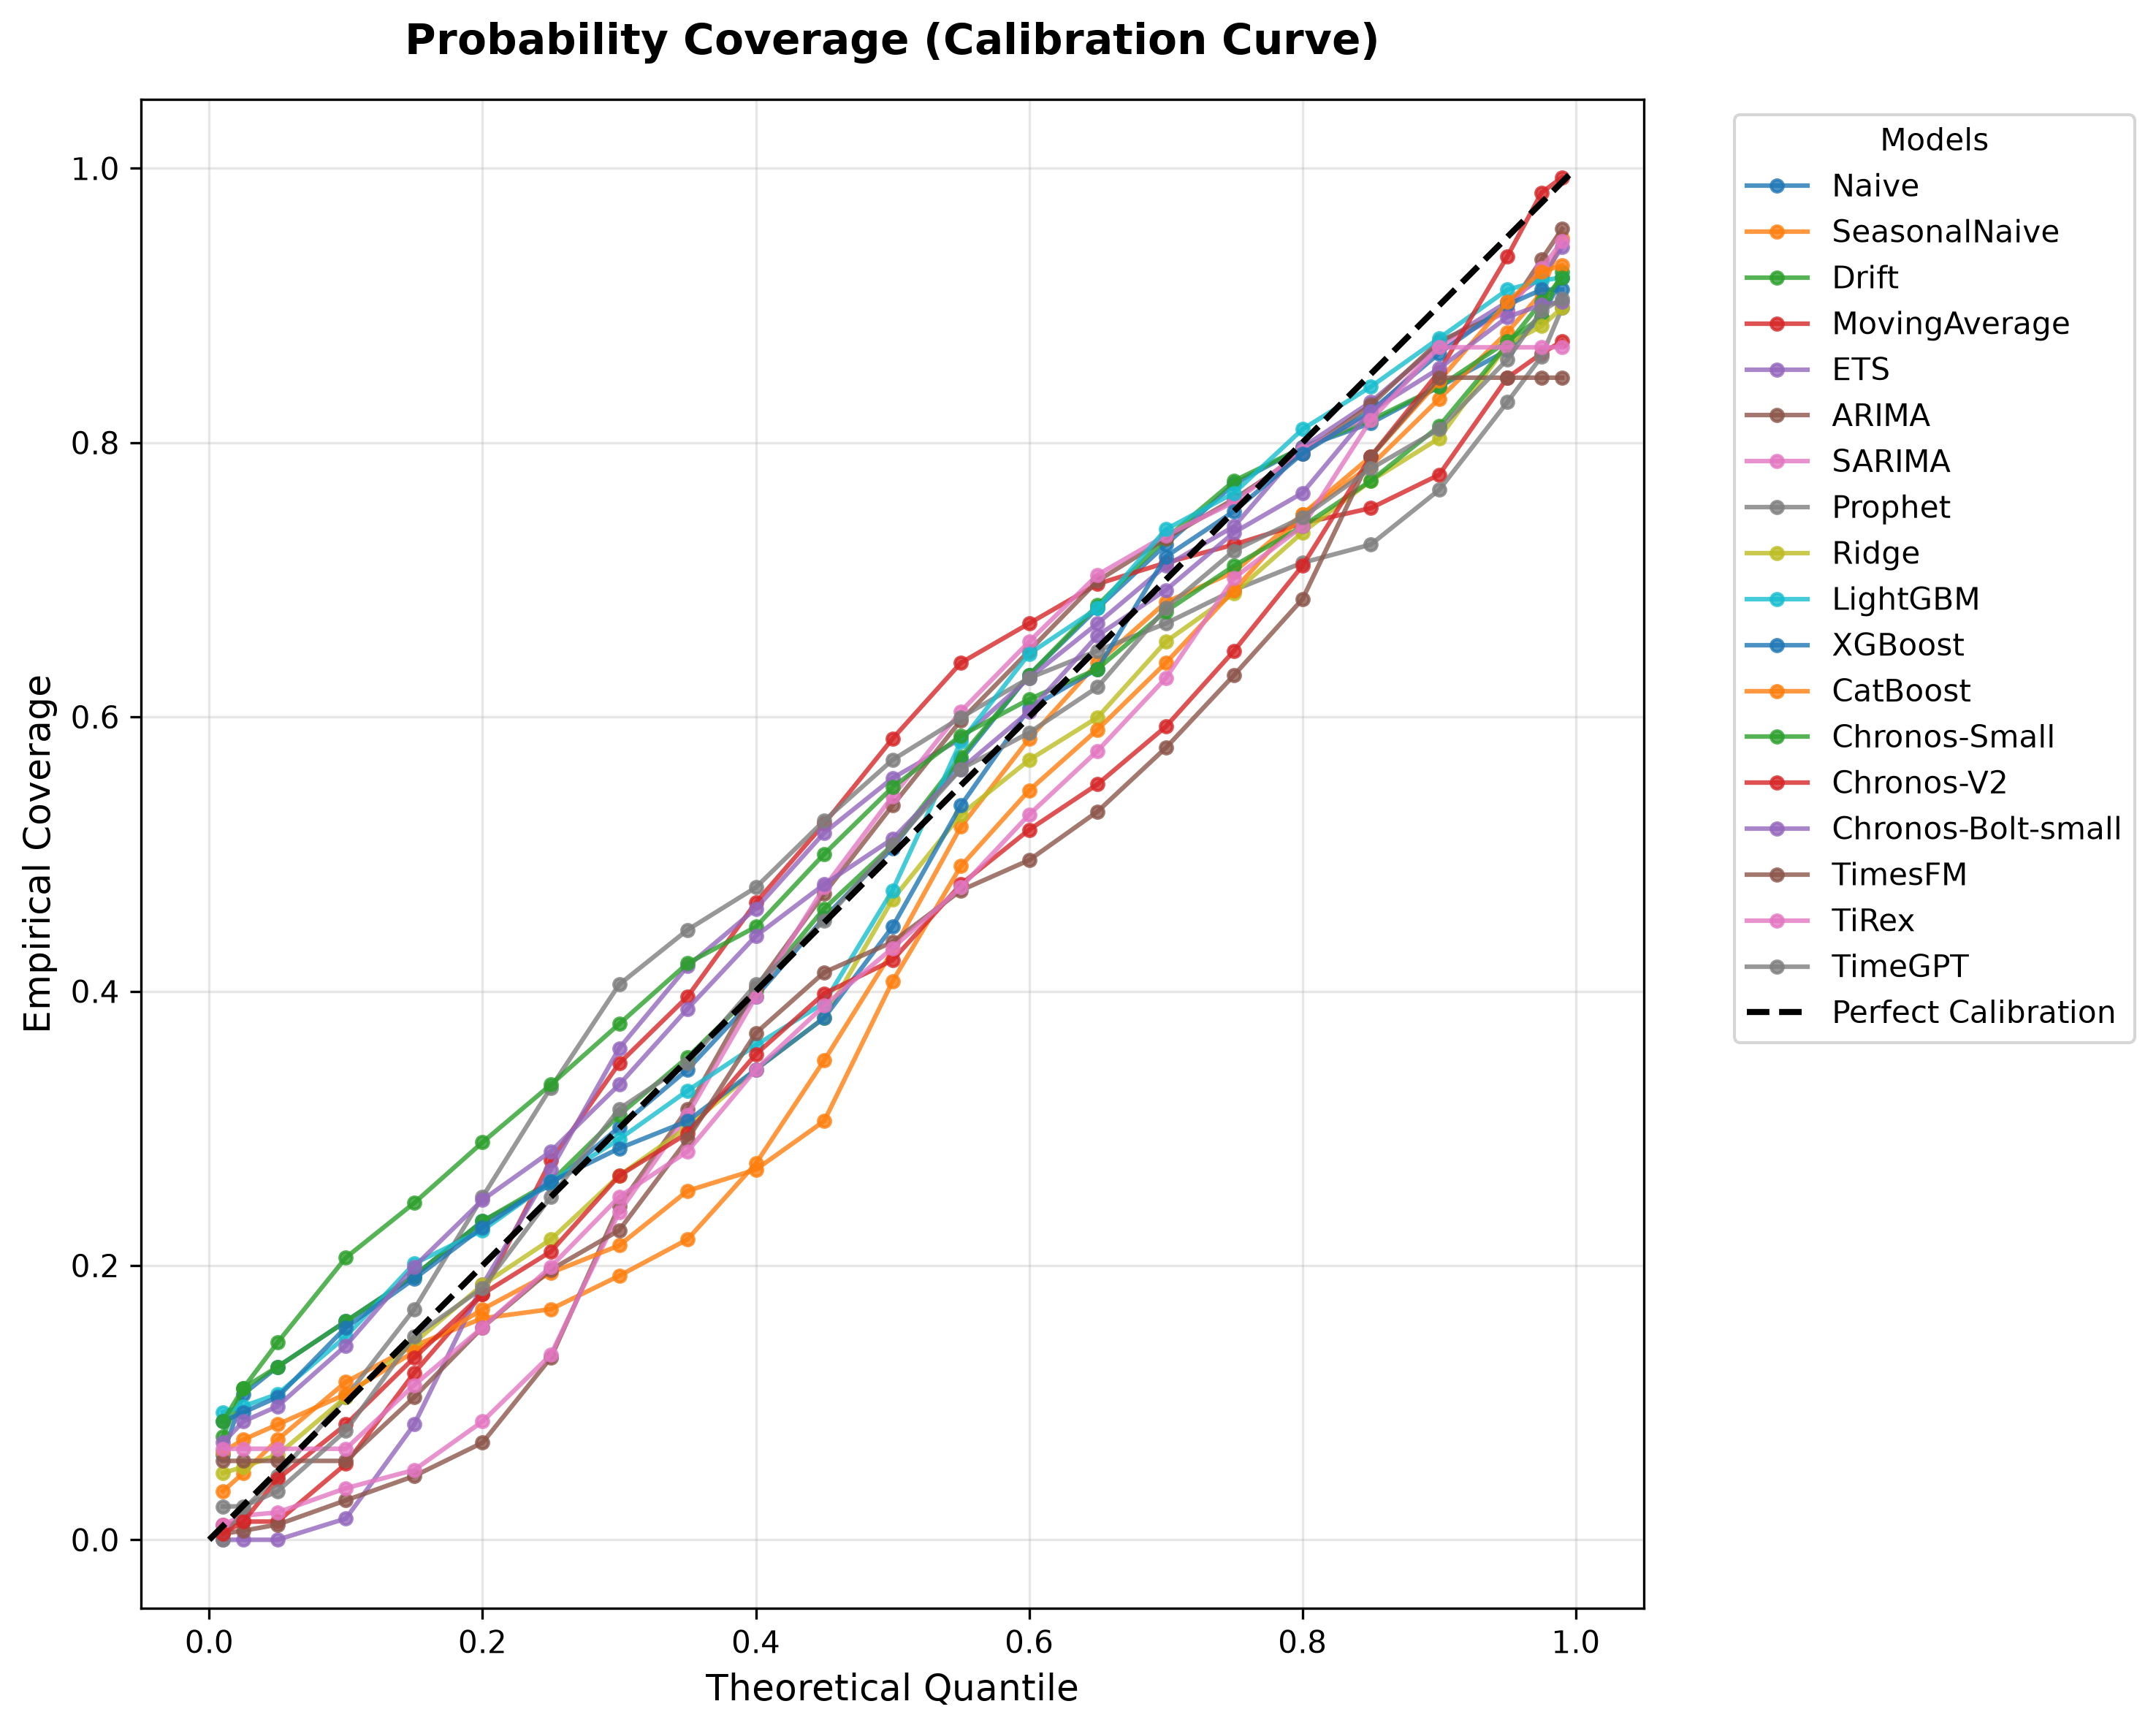
\includegraphics[width=0.9\textwidth]{results/national/plots/calibration_curve.png}
    \caption{National Probability Coverage Calibration Curves}
    \label{fig:calibration_curve}
\end{figure}

%----------------------------------------------------------------------------------------
%	SECTION 3: REGIONAL FORECASTING PERFORMANCE
%----------------------------------------------------------------------------------------

\section{Regional Forecasting Performance}

Testing forecasting models on regional data is a harder test of how well they generalize. Regional flu profiles have smaller populations. This leads to higher volatility, irregular waves, and local outbreaks. Also, regional data often has reporting delays and inconsistencies among doctor networks, creating noisy and broken time series. Our regional evaluation combines results across all 21 administrative areas in Italy over a 6-year test set (2012--2018).

%-----------------------------------
%	SUBSECTION 3.1: OVERALL REGIONAL LEADERBOARD
%-----------------------------------
\subsection{Overall Regional Leaderboard}
Table \ref{tab:regional_leaderboard} shows the overall performance across all regional series, rolling origins, and horizons:

\begin{table}[htbp]
\centering
\caption{Aggregate Regional Leaderboard (Horizons 1, 2, 4, 8)}
\label{tab:regional_leaderboard}
\setlength{\tabcolsep}{4pt}
\small
\resizebox{\textwidth}{!}{%
\begin{tabular}{lccccccc}
\hline
\textbf{Model} & \textbf{MAE} & \textbf{WIS} & \textbf{RMSE} & \textbf{sMAPE} & \textbf{MASE} & \textbf{Pinball Loss} & \textbf{95\% Cov. Dist.} \\ \hline
\textbf{TimesFM} & \textbf{2.2835} & 1.6262 & 3.5689 & 62.3821 & \textbf{0.9831} & 0.8131 & 0.1929 \\
\textbf{Chronos-V2} & 2.3677 & \textbf{1.5588} & 3.6270 & 63.6049 & 1.0234 & \textbf{0.7794} & \textbf{0.0355} \\
\textbf{TiRex} & 2.4424 & 1.7422 & 3.8159 & 65.8391 & 1.0496 & 0.8711 & 0.1780 \\
\textbf{Chronos-Bolt-Small} & 2.4826 & 1.6944 & 3.6648 & 64.8554 & 1.0598 & 0.8472 & 0.0998 \\
\textbf{TimeGPT} & 2.6128 & 1.9001 & 3.8929 & 66.0471 & 1.1119 & 0.9501 & 0.0842 \\
\textbf{CatBoost} & 2.8264 & 2.0565 & 4.0187 & 68.5128 & 1.2131 & 1.0282 & 0.1016 \\
\textbf{ARIMA} & 2.8408 & 1.9731 & 4.1156 & 69.2503 & 1.2123 & 0.9865 & 0.0908 \\
\textbf{Ridge} & 2.8706 & 2.0787 & 4.0579 & 72.4383 & 1.2048 & 1.0394 & 0.1230 \\
\textbf{SARIMA} & 2.8747 & 2.0001 & 4.1921 & 70.0072 & 1.2214 & 1.0000 & 0.0903 \\
\textbf{XGBoost} & 3.0347 & 2.2395 & 4.3832 & 71.4110 & 1.2797 & 1.1198 & 0.1124 \\
\textbf{Naive} & 3.1394 & 2.3587 & 4.7436 & 65.4318 & 1.3402 & 1.1793 & 0.1097 \\
\textbf{ETS} & 3.1534 & 2.2594 & 4.6893 & 70.5525 & 1.3524 & 1.1297 & 0.0717 \\
\textbf{Drift} & 3.1880 & 2.3932 & 4.8128 & 72.4303 & 1.3601 & 1.1966 & 0.1106 \\
\textbf{LightGBM} & 3.1956 & 2.2824 & 4.3795 & 73.6414 & 1.3600 & 1.1412 & 0.1235 \\
\textbf{MovingAverage} & 3.5649 & 2.4731 & 4.7971 & 78.4599 & 1.5221 & 1.2366 & 0.1143 \\
\textbf{Prophet} & 3.8794 & 2.7046 & 5.4127 & 83.0651 & 1.6408 & 1.3523 & 0.1491 \\
\textbf{SeasonalNaive} & 4.7138 & 3.2793 & 6.6037 & 100.3422 & 1.9877 & 1.6396 & 0.1030 \\ \hline
\end{tabular}%
}
\end{table}

Consistent with the national results, the top five regional models are zero-shot foundation models. On regional data, \textbf{TimesFM} achieves the lowest overall MAE (\textbf{2.2835}), followed closely by \textbf{Chronos-V2} (MAE 2.3677).

This regional accuracy is shown in Figure \ref{fig:regional_performance_mae}, which displays the average MAE per region for each model. The plot highlights that TimesFM and Chronos-V2 perform well in both large northern regions (like Lombardy and Piedmont) and smaller southern regions (like Puglia and Sicily). This shows consistent performance regardless of population size.

To understand these results, we can look at the differences between the top two models:
\begin{itemize}
    \item \textbf{Why TimesFM Leads in Point Accuracy (MAE):} TimesFM's patch design groups adjacent weeks into non-overlapping blocks (patches). This patching mechanism works like a local filter, smoothing out high-frequency noise and reporting errors. By modeling relationship patterns between patches instead of individual noisy data points, TimesFM generalizes well over volatile regional changes.
    \item \textbf{Why Chronos-V2 Leads in Calibration (WIS):} Although TimesFM has the lowest point error, it is too confident. Its 95\% prediction interval only covers \textbf{75.86\%} of the data (Coverage Distance of \textbf{0.1929}). In contrast, Chronos-V2 has a Coverage Distance of only \textbf{0.0355}, which means its actual coverage is \textbf{94.51\%} (and it achieves the lowest overall WIS of \textbf{1.5588}). Chronos-V2's softmax sampling lets it output wider, asymmetric intervals that reflect high regional volatility. In contrast, TimesFM's decile interpolation underestimates uncertainty.
\end{itemize}

This calibration gap is a problem for regional health planning. Underestimating the upper bounds of cases can lead to poor planning for hospital capacity.

\begin{figure}[H]
    \centering
    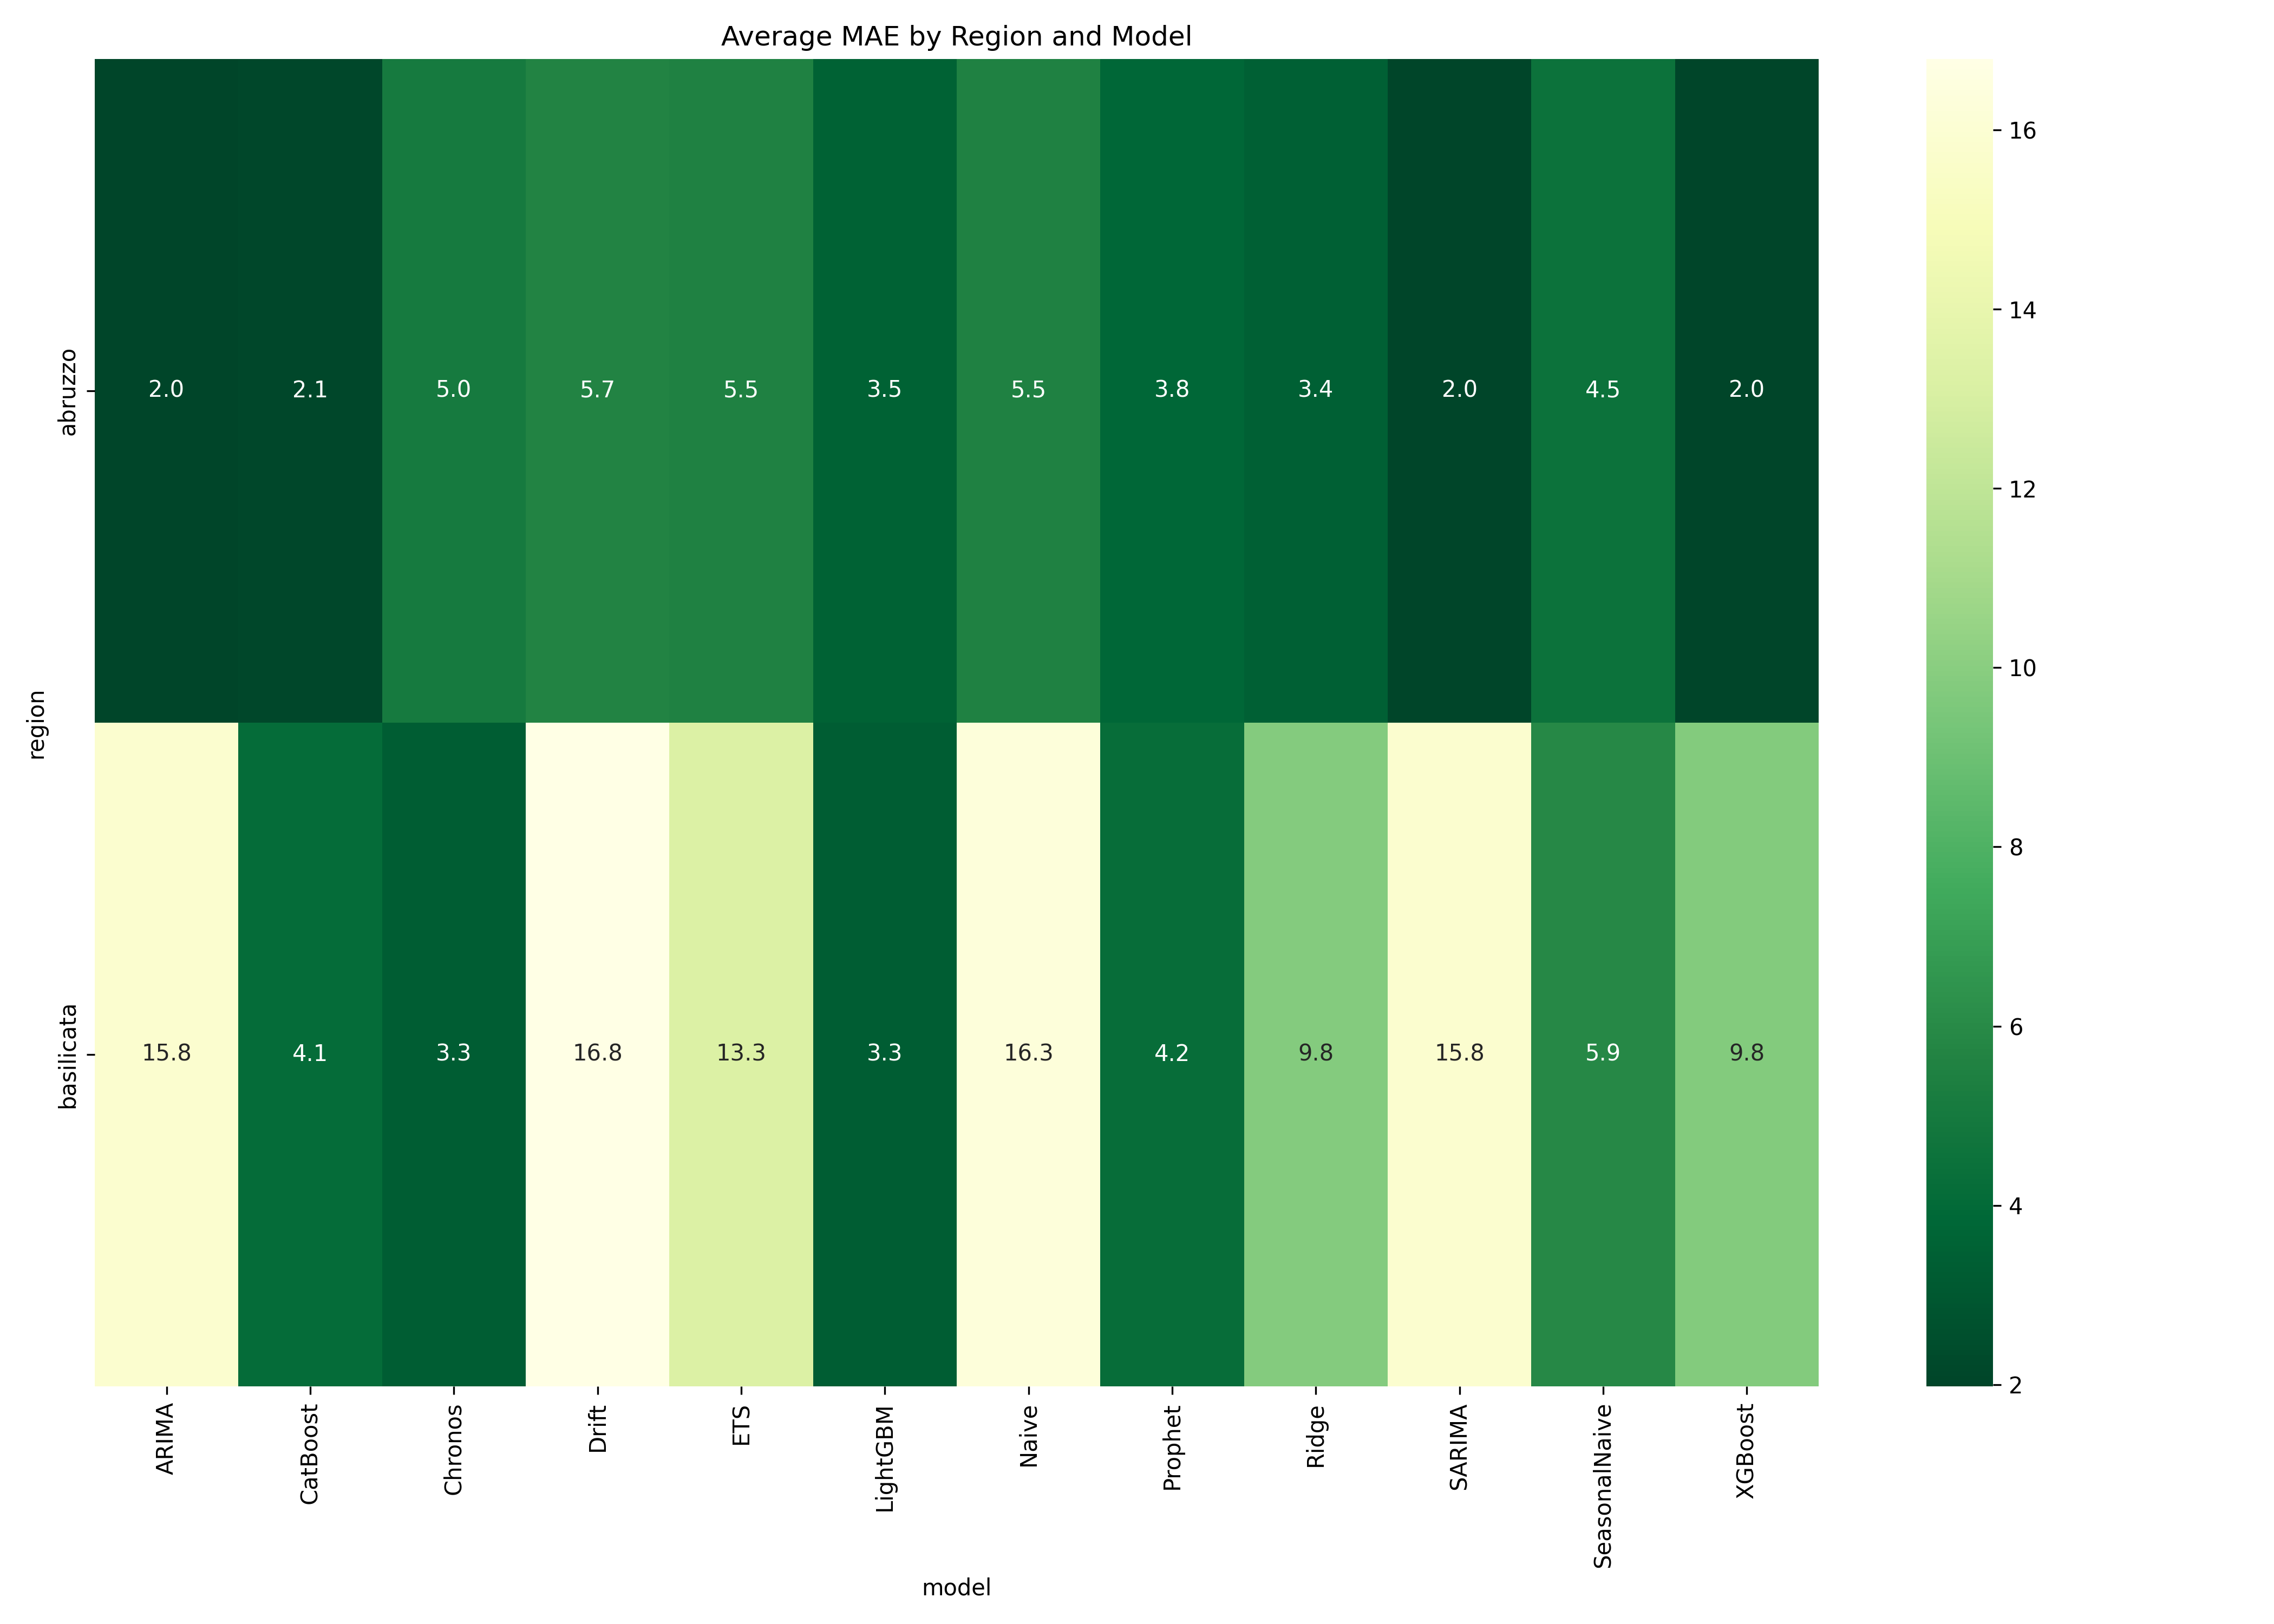
\includegraphics[width=0.9\textwidth]{results/regional/plots/regional_performance_mae.png}
    \caption{Regional Forecasting Performance (Mean MAE per Region and Model)}
    \label{fig:regional_performance_mae}
\end{figure}

%-----------------------------------
%	SUBSECTION 3.2: REGIONAL WIN BREAKDOWN
%-----------------------------------
\subsection{Regional Win Breakdown}
A region-by-region breakdown of the best model (using the lowest MAE) shows the complete dominance of the zero-shot approach:

\begin{itemize}
    \item \textbf{TimesFM (13 wins):} Dominates in major regions including Lombardy (MAE 2.11), Piedmont (MAE 2.10), Emilia-Romagna (MAE 2.37), Veneto (MAE 1.79), and regional areas like Valle d'Aosta (MAE 3.28), Marche (MAE 3.10), Abruzzo (MAE 2.62), Basilicata (MAE 2.19), Liguria (MAE 2.00), Sardinia (MAE 1.97), Umbria (MAE 3.09), PA Bolzano (MAE 2.27), and PA Trento (MAE 2.16).
    \item \textbf{Chronos-Bolt-Small (3 wins):} Calabria (MAE 1.69), Sicily (MAE 1.64), and Tuscany (MAE 2.29).
    \item \textbf{Chronos-V2 (2 wins):} Lazio (MAE 1.65) and Puglia (MAE 1.91).
    \item \textbf{TimeGPT (2 wins):} Campania (MAE 2.75) and Friuli-Venezia Giulia (MAE 2.01).
    \item \textbf{TiRex (1 win):} Molise (MAE 2.04).
\end{itemize}

None of the traditional statistical models or supervised machine learning models got the lowest error in any of the 21 regions. This suggests that pre-trained zero-shot foundation models are better at adapting to local, high-noise data:
\begin{itemize}
    \item \textbf{Overfitting in Local Models:} Locally trained models (like GBDTs or ARIMA) suffer from unstable parameters and overfitting when trained on short, noisy regional data. They struggle to separate the true transmission signal from reporting noise.
    \item \textbf{Generalization of Global Priors:} Zero-shot foundation models do not train on the target regional data. By applying general priors learned during pre-training on diverse datasets, they predict stable trends that are not affected by local reporting noise.
\end{itemize}

To show these regional wins on a map without using complex GIS libraries (like geopandas or shapely) that often break in cloud environments, our code (in \texttt{src/utils/visualizations.py}) creates a custom grid map of Italy (shown in Figure \ref{fig:best_model_map}). It places each region in a 2D grid that represents the shape of the country. This layout allows for quick geographic analysis of model performance. It highlights that neighboring regions often share similar top-performing models due to geographic similarities in disease spread.

\begin{figure}[H]
    \centering
    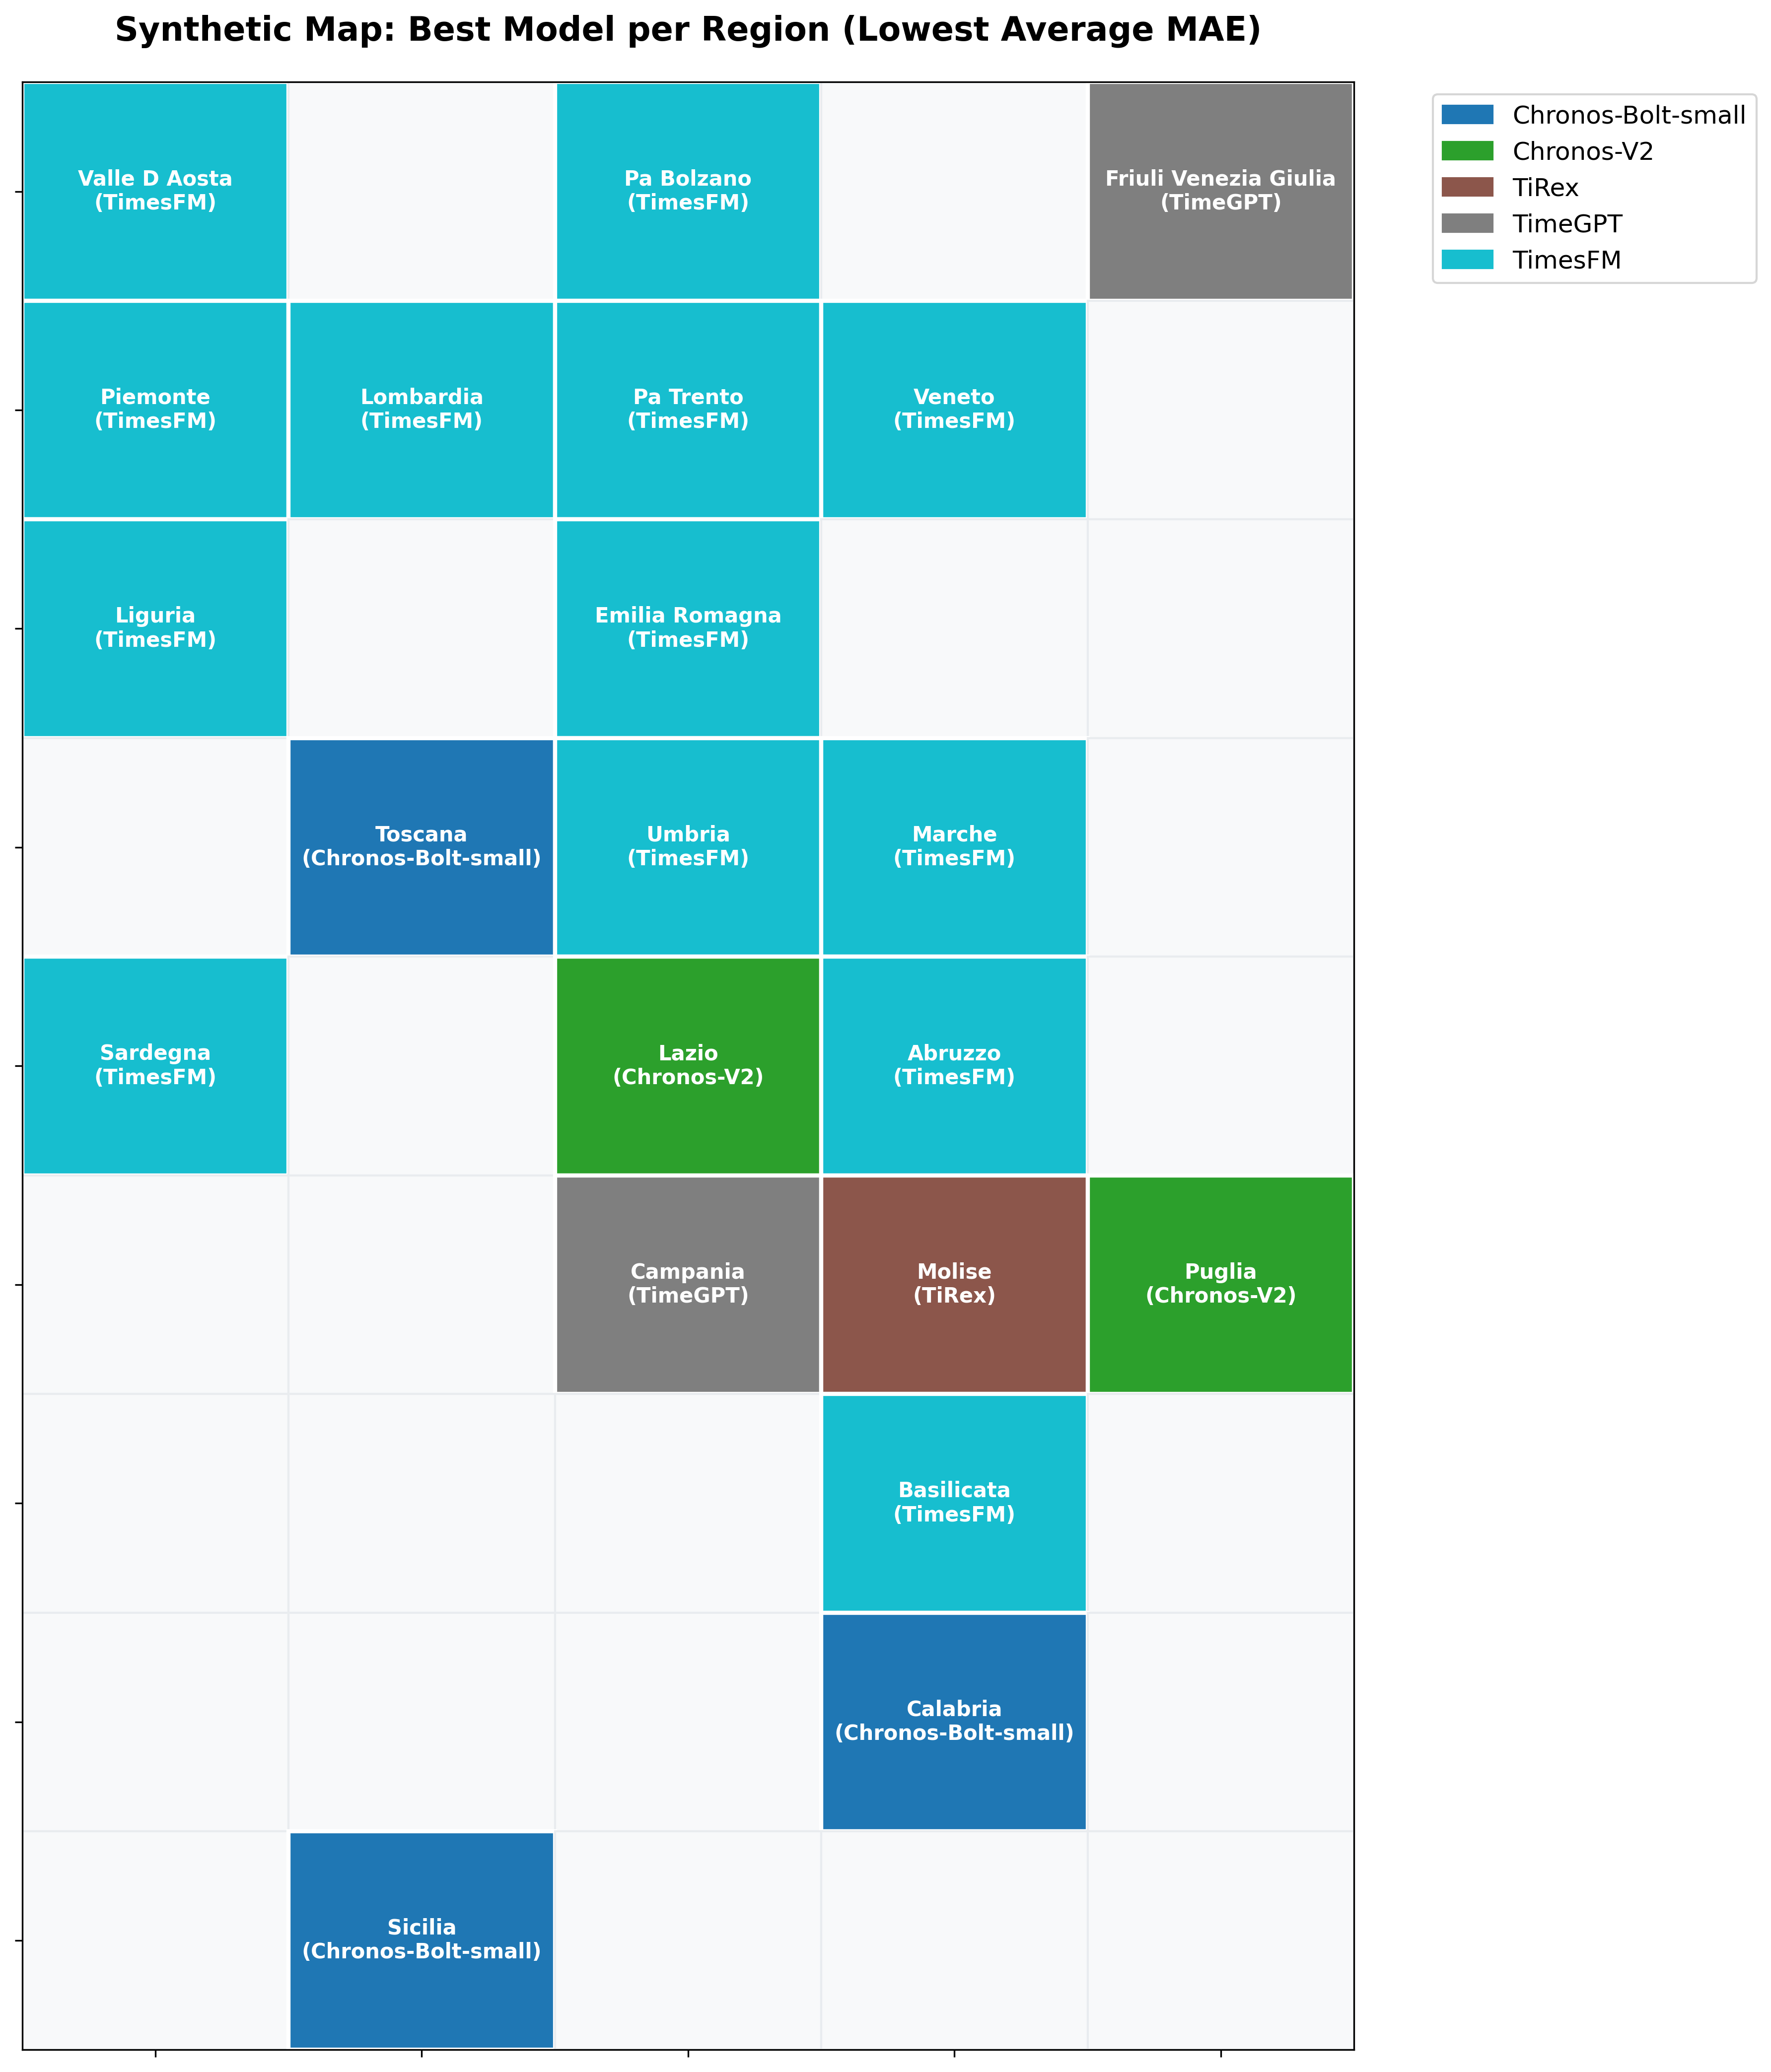
\includegraphics[width=0.9\textwidth]{results/regional/plots/best_model_map.png}
    \caption{Geographic Distribution of the Best Forecasting Model per Region in Italy}
    \label{fig:best_model_map}
\end{figure}

%----------------------------------------------------------------------------------------
%	SECTION 4: SEASONAL PEAK FORECASTING PERFORMANCE
%----------------------------------------------------------------------------------------

\section{Seasonal Peak Forecasting Performance}

Predicting the seasonal peak accurately is one of the most important goals in disease forecasting. It tells us when and how large the peak demand for healthcare will be. We evaluate models on how well they predict peak timing (timing error in weeks) and peak size (absolute and relative percentage errors) during the surveillance window (October 1st to June 1st).

%-----------------------------------
%	SUBSECTION 4.1: NATIONAL PEAK FORECASTING
%-----------------------------------
\subsection{National Peak Forecasting}
Table \ref{tab:national_peak_errors} summarizes peak forecasting errors at the national level. It shows results for the newest forecast configuration (``latest'') and at a fixed 4-week horizon ($h=4$):

\begin{table}[htbp]
\centering
\caption{National Peak Forecasting Errors (Timing in Weeks, Intensity in \%)}
\label{tab:national_peak_errors}
\setlength{\tabcolsep}{6pt}
\small
\resizebox{\textwidth}{!}{%
\begin{tabular}{lcccc}
\hline
\textbf{Model} & \textbf{Latest PTE (weeks)} & \textbf{Latest Rel. PIE (\%)} & \textbf{H4 PTE (weeks)} & \textbf{H4 Rel. PIE (\%)} \\ \hline
ARIMA & 1.00 & 13.28\% & 2.24 & 27.10\% \\
SARIMA & 1.06 & 11.19\% & 2.47 & 22.72\% \\
\textbf{Chronos-Small} & 1.53 & 16.83\% & 3.41 & 25.66\% \\
\textbf{Chronos-Bolt-Small} & 1.65 & 27.20\% & 3.06 & 34.12\% \\
\textbf{Chronos-V2} & 1.88 & 18.67\% & 3.41 & 30.55\% \\
\textbf{TiRex} & 1.88 & 20.55\% & 3.65 & 35.30\% \\
\textbf{TimesFM} & 2.47 & 19.72\% & 4.00 & 33.88\% \\
CatBoost & 1.82 & 31.48\% & 3.65 & 45.80\% \\ \hline
\end{tabular}%
}
\end{table}

\subsubsection{The Peak Timing Paradox}
An interesting trade-off appears from the peak evaluation: \textbf{simple statistical models (ARIMA and SARIMA) perform better than zero-shot foundation models in predicting the exact week of the peak.} In the ``latest'' configuration, ARIMA predicts the peak week with an average error of only \textbf{1.00 week}. SARIMA achieves a relative size error of just \textbf{11.19\%}. Among the foundation models, Chronos-Small performs best (1.53 weeks timing error), while TimesFM has a larger timing error (2.47 weeks). At 4 weeks ahead, ARIMA and SARIMA keep their lead, predicting the peak timing within 2.24 and 2.47 weeks. In contrast, Chronos-V2 has a timing error of 3.41 weeks.

This ``Peak Timing Paradox'' is caused by the differences between local statistical fitting and zero-shot curve matching:
\begin{itemize}
    \item \textbf{Local Autoregressive Calibration:} Classical models (ARIMA and SARIMA) are trained directly on the active season data. Their training objective minimizes prediction errors on the local history. This makes their coefficients ($\phi_1, \dots, \phi_p$) highly sensitive to immediate changes in the speed of transmission. Also, because their time index is linked to actual calendar dates, they benefit from the strong seasonal patterns in the historical data (where peaks usually occur between ISO Week 52 and ISO Week 6).
    \item \textbf{Zero-Shot Curve-Matching shifts:} Foundation models, by contrast, make predictions based on geometric shape matching. Because they run in a zero-shot setup, they do not have calendar date information or local seasonal parameters. On concatenated active weeks, the models see a continuous wave. While this keeps the wave shape intact, it removes the calendar context. During forecasting, the models can shift the predicted curve forward or backward by a few weeks (a phase shift). This increases their Peak Timing Error (PTE) even if their overall point accuracy (MAE/RMSE) remains very high.
\end{itemize}

This trade-off is shown in Figure \ref{fig:peak_performance_scatter}. This plot compares each model's timing error against its size error for the newest predictions. ARIMA and SARIMA sit closest to the origin, showing both low timing and size errors. Foundation models form a wider cluster. They predict the peak size reasonably well but have a larger variance in timing because they lack calendar dates.

\begin{figure}[H]
    \centering
    \includegraphics[width=0.9\textwidth]{results/national/plots/peak_performance_scatter.png}
    \caption{National Peak Forecasting Performance: Timing vs Intensity Errors}
    \label{fig:peak_performance_scatter}
\end{figure}

\subsubsection{Case Study: Peak Capture in the 2023--2024 Season}
To see how these averages translate to real-world planning, Figure \ref{fig:peak_capture_example} shows predictions made on October 29, 2023 (red dotted line), at the start of the growth phase of the 2023--2024 season. During this season, flu cases reached a record high of over 18.0 per 1000 assisted, peaking in late December 2023.

Looking at the predicted paths from this early date:
\begin{itemize}
    \item \textbf{High-responsiveness Models:} Classical models (ARIMA, SARIMA) and machine learning models (XGBoost, LightGBM) predict a rapid, steep climb to about 13.0 cases per 1000 at the end of the 8-week horizon. Among zero-shot foundation models, \textbf{Chronos-V2} projects a steady upward trend that matches the initial slope of the real curve, reaching about 10.6 cases per 1000. This shows that the zero-shot classification design reacts quickly to the start of a wave.
    \item \textbf{Conservative Foundation Models:} Other foundation models, like \textbf{TimesFM} and \textbf{TiRex}, are more cautious. They predict a slower rise (reaching ~8.5 and ~7.1 respectively), underestimating the speed and height of the wave.
    \item \textbf{Flat-line and Declining Baselines:} Baselines like Naive (flat at ~5.2), Moving Average, and Seasonal Naive fail completely to predict the peak. Prophet and CatBoost also fail to project the upward trend, showing either a flat line or a premature decline.
\end{itemize}
This comparison shows that while some models look good on average historical tests, their real usefulness for public health depends on their sensitivity to early-wave growth. Chronos-V2 balances strong overall accuracy with a quick response to upcoming peaks, while other models show a conservative bias that could delay hospital staffing alerts.

\begin{figure}[H]
    \centering
    \includegraphics[width=0.95\textwidth]{results/national/plots/national_peak_capture_2023.png}
    \caption{National Forecast Comparison: Capture Peak from Origin 2023-10-29}
    \label{fig:peak_capture_example}
\end{figure}

%-----------------------------------
%	SUBSECTION 4.2: REGIONAL PEAK FORECASTING
%-----------------------------------
\subsection{Regional Peak Forecasting}
Table \ref{tab:regional_peak_errors} summarizes peak timing and size errors averaged across all 21 regional entities:

\begin{table}[htbp]
\centering
\caption{Regional Peak Forecasting Errors (Timing in Weeks, Intensity in \%)}
\label{tab:regional_peak_errors}
\setlength{\tabcolsep}{10pt}
\small
\resizebox{\textwidth}{!}{%
\begin{tabular}{lcc}
\hline
\textbf{Model} & \textbf{Latest PTE (weeks)} & \textbf{Latest Rel. PIE (\%)} \\ \hline
Naive & 3.18 & 77.59\% \\
ARIMA & 3.76 & 53.67\% \\
SARIMA & 4.12 & 60.19\% \\
\textbf{Chronos-Bolt-Small} & 4.15 & 54.36\% \\
\textbf{Chronos-V2} & 4.87 & 58.09\% \\
\textbf{TiRex} & 3.98 & 57.22\% \\
\textbf{TimesFM} & 4.10 & 54.94\% \\
CatBoost & 4.67 & 70.92\% \\ \hline
\end{tabular}%
}
\end{table}

At the regional level, peak timing errors increase for all models. This is due to high noise, irregular wave shapes, and double peaks in small regional populations. In this noisy environment, the difference between local statistical models and foundation models is small. ARIMA keeps a slight lead in timing error (\textbf{3.76 weeks}), followed closely by TiRex (\textbf{3.98 weeks}), TimesFM (\textbf{4.10 weeks}), and Chronos-Bolt-Small (\textbf{4.15 weeks}).

The naive model's low timing error (3.18 weeks) is a baseline artifact rather than real forecasting ability. We call this the \textbf{Naive Peak Alignment Artifact}:
\begin{itemize}
    \item \textbf{Mathematical Formulation:} Since the Naive model projects the last value forward ($\hat{y}_{t_0+h \mid t_0} = y_{t_0}$), its predicted peak is locked to the value at the forecast date ($t_0$). As the forecast date rolls through the winter weeks, it passes close to the real peak week. When this happens, the model's flat prediction naturally aligns with the peak timing, which artificially lowers the timing error.
    \item \textbf{Size Degradation:} Although the Naive model gets a low timing error of \textbf{3.18 weeks} because of this artifact, it has a very high peak size error of \textbf{77.59\%}. It fails to predict the size of the wave, which makes it useless for planning hospital resources.
    \item \textbf{Operational Utility:} In contrast, ARIMA (53.67%), Chronos-Bolt-Small (54.36%), and TimesFM (54.94%) provide much more accurate estimates of peak height. Predicting peak size is much more useful for hospital managers when allocating ICU beds and planning clinical staff.
\end{itemize}
